%%PREAMBLE %%%%%%%%%%%%%%%%%%%%%%%%%%%%
\documentclass[10pt, a4paper]{article}% size of txt = 10pt
\usepackage[top= 2cm,
			bottom = 2cm,
			left = 1.7cm,
			right = 1.7cm,
			footskip = 0.5cm,
			headsep = 0cm,
			headheight = 0cm
					]{geometry}
\usepackage{amsmath} % math packages
\usepackage{amsfonts}% math packages
\usepackage{amssymb} % math packages
\usepackage{graphicx} %package for including graphics
\usepackage{array}
\usepackage[thinlines]{easytable}
\usepackage{float}
\usepackage[section]{placeins}
\usepackage[hidelinks]{hyperref}
\usepackage[shortlabels]{enumitem}
\usepackage{svg}
\usepackage{bigstrut}
\usepackage{wrapfig,lipsum,booktabs}
\usepackage{subcaption}
\usepackage{xfrac}
\usepackage{pdfpages}
\usepackage{listings}
\usepackage{xcolor}


\usepackage{listings}
\usepackage{color} %red, green, blue, yellow, cyan, magenta, black, white
\definecolor{mygreen}{RGB}{28,172,0} % color values Red, Green, Blue
\definecolor{mylilas}{RGB}{170,55,241}

\definecolor{codegreen}{rgb}{0,0.6,0}
\definecolor{codegray}{rgb}{0.5,0.5,0.5}
\definecolor{codepurple}{rgb}{0.58,0,0.82}
\definecolor{backcolour}{rgb}{1,1,1}

\lstdefinestyle{mystyle}{
    backgroundcolor=\color{backcolour},   
    commentstyle=\color{codegreen},
    keywordstyle=\color{magenta},
    numberstyle=\tiny\color{codegray},
    stringstyle=\color{codepurple},
    basicstyle=\ttfamily\footnotesize,
    breakatwhitespace=false,         
    breaklines=true,                 
    captionpos=b,                    
    keepspaces=true,                 
    numbers=left,                    
    numbersep=5pt,                  
    showspaces=false,                
    showstringspaces=false,
    showtabs=false,                  
    tabsize=2
}
\lstset{style=mystyle}


%date format
\def\mydate{\leavevmode\hbox{\twodigits\day.\twodigits\month.\the\year}}
\def\twodigits#1{\ifnum#1<10 0\fi\the#1}

\usepackage{indentfirst}
\setlength{\parindent}{1cm}

\makeatletter
\newcommand{\thickhline}{%
    \noalign {\ifnum 0=`}\fi \hrule height 2pt
    \futurelet \reserved@a \@xhline
}
\newcolumntype{"}{@{\hskip\tabcolsep\vrule width 2pt\hskip\tabcolsep}}
\makeatother
\newcolumntype{?}{!{\vrule width 2pt}}
%%DOC ENVIROMENT%%%%%%%%%%%%%%%%%%%%%%%
\begin{document}
%Title 
\begin{flushleft}%% left justification
	\textbf{\Large{MKC-PKS: Úkol č. 1}}\hfill Filip Paul\\
	\large{Topologie sítí a základní aplikace \hfill\mydate}
\end{flushleft}
	\begin{enumerate}
		\item \textbf{Porovnejte vlastnosti paketových sítí s virtuálními okruhy a sítí s datagramovou službou.}\\
		\begin{figure}[ht!]
			\centering
			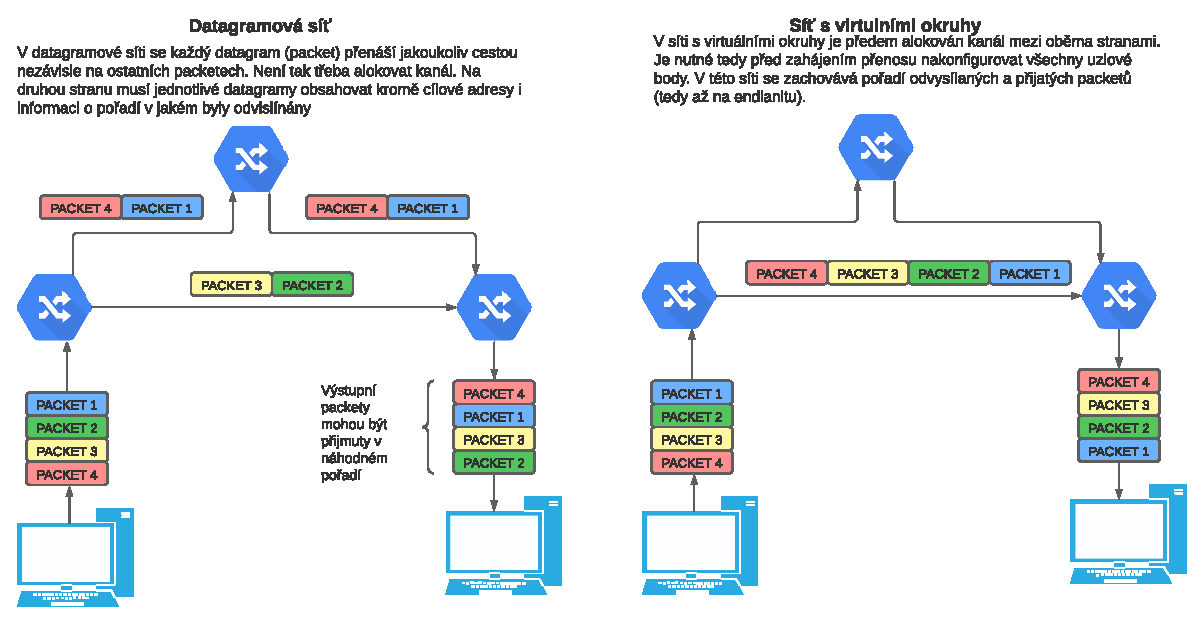
\includegraphics[width = 1\textwidth]{virtual_vs_datagram.eps}
		\end{figure}
		\item \textbf{Předpokládejte, že N = 18 uživatelů je připojeno v síti s přepínáním paketů k lince 1Mb/s. Každý 
		uživatel generuje tok 100kb/s po dobu 20\% celkového času, tj. např. v intervalu 1 hodiny je v průměru 
		aktivní po dobu 12 minut a po dobu 48 minut nevysílá\\
		Určete pravděpodobnost zahlcení odchozí linky, tj. pravděpodobnost, že současně vysílá 11 až 18
		uživatelů\\}\\
		\[P_z = \sum_{k = N_z}^{N} \binom{N}{k}p_c^k(1-p_c)^{N-k} \]\\
		\[P_z = \sum_{k = 11}^{18} \binom{18}{k}0.2^k(1-0.2)^{18-k} = 6.161956191398731e-05 \doteq  0.0062\,\% \]\\
		Výsledek byl vypočten pomocí násladujícího python scriptu:\\
		\lstinputlisting[language=python]{calc.py}
		\clearpage
		\item \textbf{Pomocí programu traceroute (tracert) určete zpoždění z vašeho počítače na server\\
		ms.urel.feec.vutbr.cz (do vypracování dejte kopii okna) Proč zpoždění neroste monotónně,
		jak postupně přibývá počet směrovačů, kterými projde testovací paket?}

		\begin{figure}[ht!]
			\centering
			\includegraphics[width = 0.8\textwidth]{tracert.PNG}
		\end{figure}

		Z výstupu programu tracert lze pozorovat, že například latence v řádku 7 a 8 (v prvním testovacím packetu)
		klesla. Nicméně nejsou zde patrné nějaké margantní změny. A latence roste s pořadím uzlu. Pokud by byla
		síť zahlcena. Zpoždění by pak záleželo převážně na zaplněnosti bufferů.
		Zajímavosí je, že pro uzel 2 a 5 program tracert zahlásil timeout a i přesto se dokázal spojit s cílovou adresou.
		Nejsem si úplně jistý proč se toto děje. Tipnul bych si, že je to kvůli tomu, že některé servery při 
		TLL = 0 packet packet pouze zahodí a nepošlou zpět žádnou zprávu ??

		Pro ukázku, kde záleží na přeplněnosti bufferů je na dalším obrázku zobrazku zobrazen tracert pro náhodnou IP adresu
		v Indii, kde se sice nepodařilo spojit až s cílovou adresou nicméně je zde patrné přepnění bufferů.	\\
		\begin{figure}[ht!]
			\centering
			\includegraphics[width = 0.8\textwidth]{tracert_INDIA.PNG}
		\end{figure}

		\clearpage
		\item\textbf{ Předpokládejte, že www prohlížeč natahuje stránku ze serveru vzdáleného 15 tis. km, která 
		obsahuje 10 obrázků po 120kB. Kapacita linky je 1Mb/s\\
		Vypočtete čas natažení celé stránky pro tyto druhy spojení:\\
		- neperzistentní\\
		- perzistentní\\
		- perzistentní + pipelining\\
		Předpokládejte nulový čas potřebný k odvysílání vlastní html stránky a příkazů, avšak uvažujte 
		skutečnou dobu nutnou k odvysílání vložených obrázků.
		Počítejte s rychlostí šíření signálu v přenosovém médiu $2\cdot10^8 m/s$ a zanedbejte případná zpoždění ve 
		směrovačích.}\\
		\begin{figure}[ht!]
			\centering
			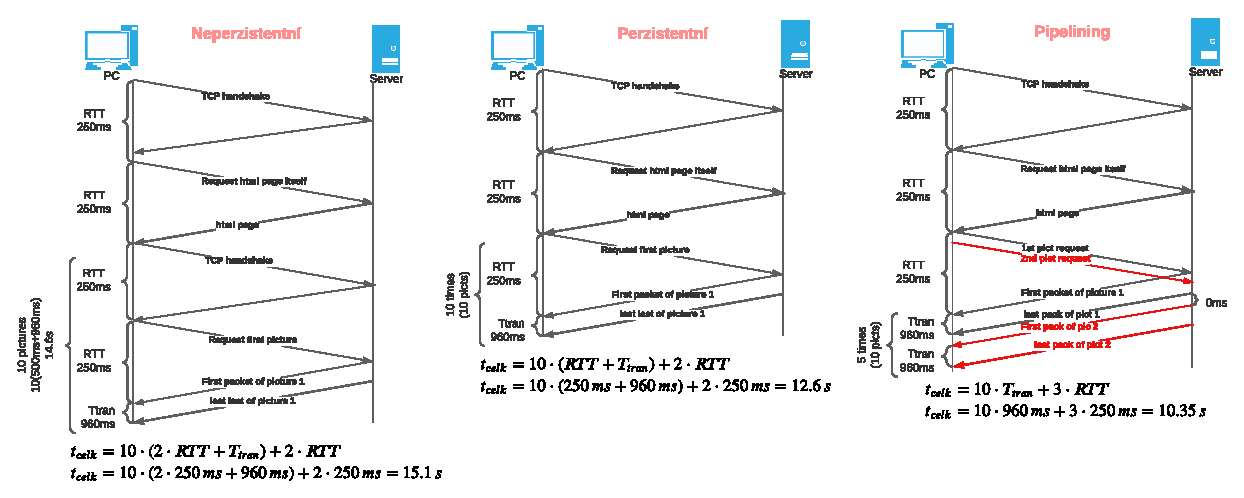
\includegraphics[width = 1\textwidth]{HTML.eps}
		\end{figure}

		
	\end{enumerate}
	

\end{document}